\documentclass[a4paper,12pt,titlepage]{article}

\title{\underline{\textbf{Machine Learning Applications in Portfolio Optimisation}}}
\author{\textit{Shaan Patankar}}
\date{\today}

\usepackage[utf8]{inputenc}
\usepackage[version=4]{mhchem}
\usepackage[dvipsnames]{xcolor}
\usepackage{fancyhdr, hyperref, tikz, tcolorbox, stmaryrd, mhchem, amssymb, amsfonts, amsmath, amsthm, setspace, fontenc, graphicx, geometry, enumitem, float, array, subcaption}

\SetSymbolFont{stmry}{bold}{U}{stmry}{m}{n}
\numberwithin{equation}{section}
\setlength{\parindent}{0pt}

\newgeometry{
	top=20mm,
	bottom=20mm,
	outer=20mm,
	inner=20mm,
}

\hypersetup{
	colorlinks=true,
	linkcolor=blue,
	citecolor=magenta,
	urlcolor=blue,
	filecolor=magenta,
	linktoc=all,
	pdftitle={Machine Learning Applications in Portfolio Optimisation},
}

\pagestyle{fancy}
\lhead{$\textbf{PORTFOLIO OPTIMISATION}$}
\rhead{$\textit{\rightmark}$}
\renewcommand{\sectionmark}[1]{\markright{#1}{}}
\cfoot{$\textbf{SHAAN PATANKAR}$}
\rfoot{$\textbf{\thepage}$}
\renewcommand{\subsectionmark}[1]{ \markright{#1}{} }
\lfoot{\empty}

%\renewcommand{\footrulewidth}{0.5pt}
%\singlespacing
%\urlstyle{same}

\begin{document}

\begin{titlepage}
	\begin{center}
		\vspace*{-3cm}
		\makebox[\textwidth]{
\includegraphics[width=\paperwidth]{Plots/UCL.png}}
		\vfill
		\vspace{3mm}
		{\LARGE\textbf{MACHINE LEARNING APPLICATIONS\\
		IN PORTFOLIO OPTIMISATION\\}}

		\vspace{0.8cm}
		by\\
		\vspace{0.8cm}

		{\LARGE\textbf{Shaan Patankar}}

		\vspace{1.5cm}
		%{\LARGE\textbf{\today}}
		\vfill
		\vspace{5cm}
		\textbf{\setstretch{2.0}
			This project centres on exploring the integration of machine learning algorithms\\
			in portfolio optimisation strategies, see the Jupyter Notebook for more info 
			}
	\end{center}
\end{titlepage}

\newpage
\tableofcontents
\pagenumbering{roman}
\thispagestyle{fancy}
\newpage

\clearpage
\pagenumbering{arabic}
\pagestyle{fancy}

\section{Background and Motivation}
\label{Background and Motivation}

Portfolio optimisation is a crucial aspect of modern finance, aiming to construct an investment 
portfolio that maximises returns while minimising risk. Traditional methods like Mean-Variance 
Optimisation ($MVO$) and the Capital Asset Pricing Model ($CAPM$) have been widely used for decades. However, 
the financial markets are complex and dynamic, and classical methods may not fully capture the 
intricate relationships between assets. \newline \par \noindent Machine learning algorithms have 
shown promise in various fields, including finance, for their ability to capture non-linear patterns 
and make data-driven decisions. This project explores the integration of machine learning algorithms 
in portfolio optimisation strategies to enhance portfolio performance and risk management.

\subsection{Research Objectives}

The main objectives of this project are as follows:

\begin{enumerate}

	\item To compare the performance of machine learning-based portfolio optimisation strategies 
		with classical $MVO$ and $CAPM$ in terms of risk-adjusted returns.

	\item To identify machine learning algorithms that are most effective in capturing non-linear 
		relationships between asset returns in a portfolio context.

	\item To investigate the impact of transaction costs, market liquidity, and model complexity on the feasibility of implementing machine 
		learning-based strategies in real-world trading scenarios.

\end{enumerate}

\section{Data Retrieval and Preprocessing}

Data retrieval and preprocessing ensure we have relevant and high-quality data for our project. This is 
vital given the financial implications of decisions based on this data. We'll utilise the \textit{Yahoo Finance} $API$ 
for fetching historical stock price data, ensuring we have a reliable and comprehensive data 
source. \newline \par \noindent For our analysis, we're more interested in the daily percentage change in stock prices (returns) 
rather than the actual prices. This gives us insights into the stocks performance and volatility. Note that raw financial data can 
have imperfections, as such, we'll address missing values and handle potential outliers by removing any empty rows to ensure data integrity
and consistency in our analysis.

\subsection{Exploratory Data Analysis (EDA)}

	After processing through all the data we can plot a stock price visualisation graph, a distribution of returns histogram,
	and a correlation heatmap (explained below). The stocks could be arbitrary, but for this project the stocks
	I've opted to look at are: $AAPL$ - Apple; $AMZN$ - Amazon; $GOOGL$ - Alphabet (\textit{Google}); 
	$MSFT$ - Microsoft; $META$ - Meta (\textit{Facebook}). \newline \par \noindent Plotting stock price trends, studying 
	the distribution of returns, and assess asset correlations provides insight and guides subsequent analyses.

	\newpage
	\begin{enumerate}

		\item The stock price visualisation plot showcases the historical stock prices for the five 
			assets over the specified time frame. The $x$-axis represents time, while the 
			$y$-axis indicates the stock price. The plot provides a clear view of the price trends 
			and allows for easy comparison between the stock performances.

			\begin{figure}[htbp] % positioning options: h=here, t=top, b=bottom, p=page of floats
				\centering
				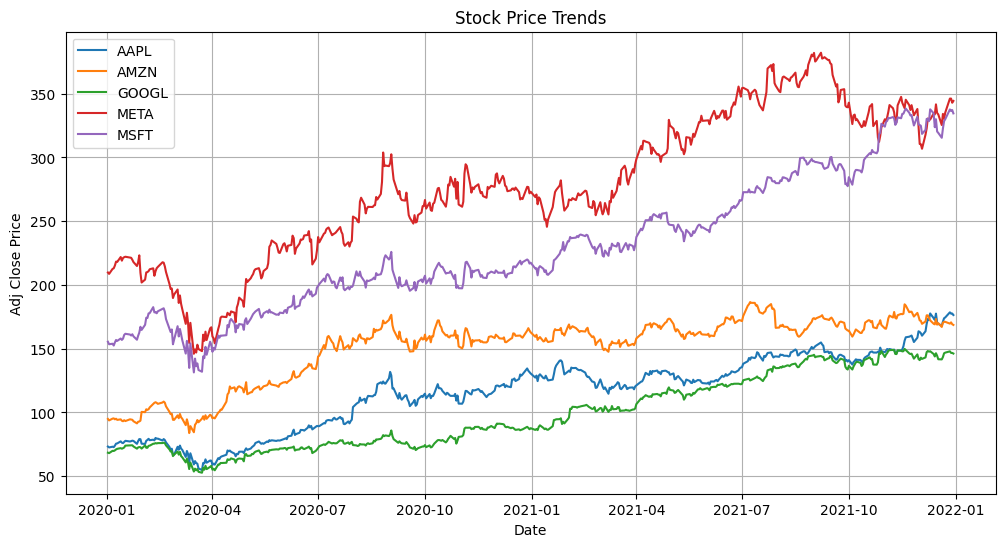
\includegraphics[width=0.8\linewidth,keepaspectratio]{Plots/StockPriceVisual.png}
				\caption{Stock price trend (\textit{Yahoo Finance})}
				\label{fig:figure1}
			  \end{figure}
			  

		\item The histogram visualises the distribution of daily returns 
			for the stocks. It offers insights into the frequency of certain return ranges, helping 
			to understand the volatility and typical performance of each asset.

			\begin{figure}[htbp] % positioning options: h=here, t=top, b=bottom, p=page of floats
				\centering
				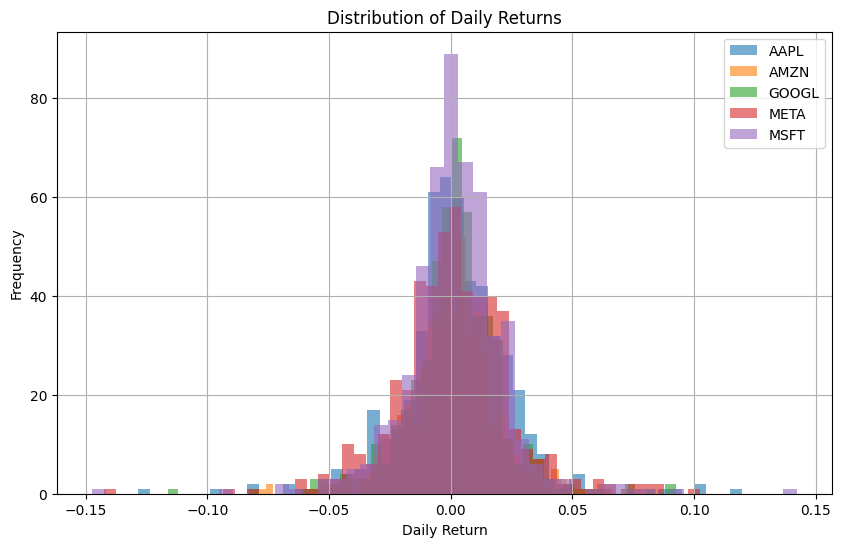
\includegraphics[width=0.8\linewidth,keepaspectratio]{Plots/HistogramVisual.png}
				\caption{Histogram of daily returns for each stock}
				\label{fig:figure2}
			  \end{figure}

		\item The heatmap displays the correlation coefficients between the daily 
			returns of the stocks. A value close to $1$ indicates a strong positive correlation, while a 
			value close to $-1$ shows a strong negative correlation. This visualisation aids in 
			understanding how different assets move in relation to each other.

			\begin{figure}[H] % positioning options: h=here, t=top, b=bottom, p=page of floats
				\centering
				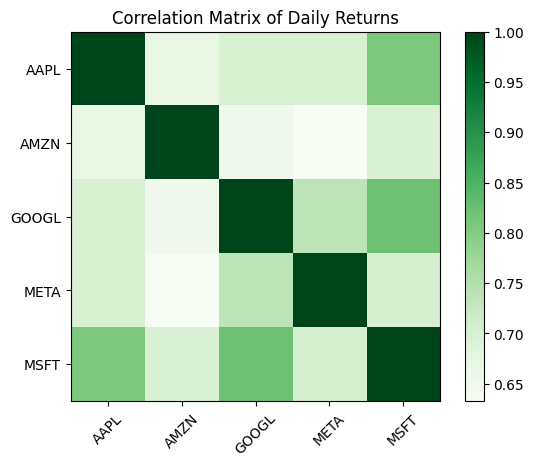
\includegraphics[scale=0.65]{Plots/HeatmapVisual.png}
				\caption{Heatmap correlation matrix of daily return}
				\label{fig:figure3}
			  \end{figure}
	
	\end{enumerate}

	\begin{tcolorbox}[colback=green!5, colframe=green!35!black, title=\textbf{Python Code}]

		Further details regarding the data collection and coding process can be found on the \textbf{Jupyter Notebook} file.

	\end{tcolorbox}

\section{Capital Asset Pricing Model (CAPM)}
\label{Capital Asset Pricing Model}

Before delving into the application of machine learning, it is essential to understand the fundamentals of 
portfolio optimisation. The following sections will provide an overview for some of the traditional portfolio optimisation methods, 
such as Mean-Variance Optimisation ($MVO$) and the Capital Asset Pricing Model ($CAPM$). \newline \par \noindent The Capital Asset Pricing 
Model ($CAPM$) is a fundamental tool in finance that relates an asset's expected return to its systematic risk. We will explore the 
concepts of beta, the security market line ($SML$), and the risk-free rate in the context of $CAPM$. The $CAPM$ uses the formula,

$$ E(R_i) = R_f + {\beta}_i (E(R_m) - R_f), $$ \par \noindent where $E(R_m)$ and $E(R_i)$ are the 
expected return of the market/asset $i$ respectively, $R_f$ is the risk-free rate, ${\beta}_i$ is the beta of asset $i$ - 
the volatility in relation to the market. Also, note that: $${\beta}_i = \frac{\text{Cov}(R_i, R_m)}{\text{Var}(R_m)},$$ \par \noindent where for
discrete random variables $X$ and $Y$ with $X_{i}$ and $Y_{i}$ denoting the $i^{th}$ sample of $X$ and $Y$ 
respectively, $\text{Var}(X) = \frac{S_{X_{i}X_{i}}}{N}$ and $\text{Cov}(X,Y) = \frac{S_{X_{i}Y_{i}}}{N}$. 
Recall that $S_{X_{i}Y_{i}} = \sum_{i=0}^{N} X_{i}Y_{i} - N \bar{X_{i}} \bar{Y_{i}}$. $\beta_{i}$ can thus 
be written as $\beta_{i} = \frac{S_{R_{i} R_{m}}}{S_{R_{m} R_{m}}}$, which is just the gradient of the 
regression line $y$ on $x$. We can use $RSS$ (or some other metric) to calculate how closely the data fits a linear model.

\subsection{Security Market Line (SML)}

The Security Market Line ($SML$) graph visually represents the relationship between the expected return of an 
asset and its systematic risk (beta). On the graph below, the $y$-axis represents the expected return of an 
asset, while the $x$-axis represents its beta. The slope of the $SML$ is determined by the market risk premium. 
Assets that plot on the $SML$ are considered fairly priced. If an asset plots above the $SML$, it indicates that 
it provides a higher return for its level of risk than the market portfolio, suggesting it might be 
undervalued. Conversely, assets below the $SML$ might be overvalued, as they offer lower returns for their 
level of risk.

\begin{figure}[htbp] % positioning options: h=here, t=top, b=bottom, p=page of floats
	\centering
	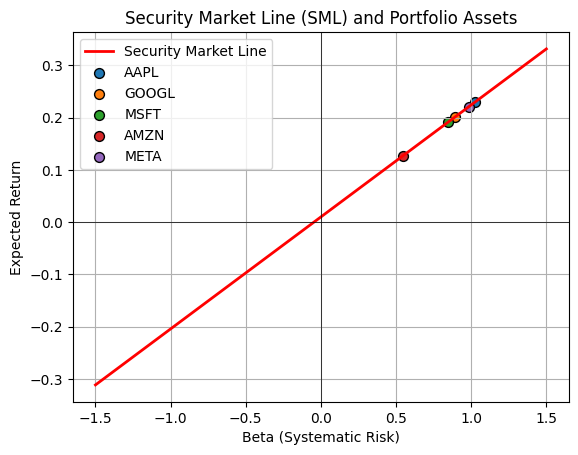
\includegraphics[width=0.8\linewidth,keepaspectratio]{Plots/SML.png}
	\caption{$SML$ and portfolio assets , $S\&P ~ 500$ is used as the market benchmark}
	\label{fig:figure4}
  \end{figure}

\par \noindent In this plot we've taken market data from each of the assets and the $S\&P ~ 500$ which acts as the market benchmark. 
By taking the \texttt{risk\_free\_rate} at $1\%$ (details in the Notebook), calculating the \texttt{expected\_stock\_return} and 
\texttt{expected\_market\_return}, we can use this to find the \texttt{market\_risk\_premium} which is the slope of the $SML$ (red line)
using the $CAPM$ formula, \texttt{market\_risk\_premium = expected\_market\_return - risk\_free\_rate}. Multiplying the market risk 
premium by $\beta_{i}$ and adding the risk free rate will give us the expected return for each of the assets (see below).

\subsection{Asset Beta and Expected Returns}

A beta value greater than $1$ suggests that the asset's returns are more volatile than the market's. In Apple's case, 
its beta, $1.0264$, suggests that it's roughly $2.64\%$ more volatile than the market. The $CAPM$ suggests that, given 
Apple's beta and the prevailing market conditions, an investor should expect a return of approximately $22.99\%$ for holding 
Apple, given the risk associated.\newline \par \noindent Google's beta ($0.8918$) suggests that it's about $10.82\%$ 
less volatile than the market. For the risk associated with holding Google (which is slightly less than the market risk), 
an investor might expect a return of $20.11\%$. Microsoft is about $15.18\%$ less volatile than 
the market having a beta of $0.8482$. Given this beta value, we'd expect a return of $19.17\%$ for 
holding it. \newline \par \noindent Amazon's low beta $0.5479$ suggests it's approximately $45.21\%$ less volatile than the 
market. This might seem surprising given Amazon's growth, but it could be influenced by time frame or some of the 
assumptions/limitations of $CAPM$, we will discuss some of these drawbacks later in the section. Amazon's expected return 
is the lowest among the assets ($12.74\%$), reflecting its lower beta. \newline \par \noindent Meta's beta value of $0.9852$ 
suggests its returns are roughly in line with the market, being just $1.48\%$ less volatile, with expected returns similar to Apple 
of $22.11\%$. \newline \par \noindent Some of these expected returns are unreasonably high, and comparing with the actual historical returns
for each asset we can see that the models predictions are not very accurate. Next, we will explore possible reasons as to why the model is 
predicting higher expected returns.

\subsection{Assumptions and Limitations of CAPM}

	Here are some of the assumptions made when using the Capital Asset Pricing Model, these assumptions
	simplify our model - making it easier to use; however, this comes at the cost of making the model 
	unrealistic/impractical in real-world scenarios. 

	\begin{enumerate}
		
		\item Investors hold diversified portfolios: this implies that investors will only require a 
			return for the systematic risk of their investments.

		\item No transaction costs: investors can buy and sell securities without incurring any costs, 
			which isn't the case in real-world scenarios.

		\item Investors can lend and borrow at the risk-free rate: this is often not feasible in 
			real markets.
		
		\item All investors have the same expectations: investors are assumed to agree on the expected 
			returns, volatilities, and correlations of all assets.
	
	\end{enumerate}
	
	Here are a list of the limitations of the Capital Asset Pricing Model, these limitations are a direct
	result of some of the simplification/assumptions we have made when using the model. These limitations 
	naturally suggests to us to use machine learning models which we will explore in the later sections.

	\begin{enumerate}

		\item Beta's predictive power: the beta of $CAPM$, which measures systematic risk, may not 
			always be a complete measure of risk.
		
		\item Market portfolio: the true market portfolio cannot be observed in reality, so 
			proxies like the $S\&P ~ 500$ are used, which might not capture the entire market.
			
		\item Static nature: $CAPM$ is a single-period model and doesn't capture changes over 
			multiple periods.
	
	\end{enumerate}
		
	Again, machine learning can help in capturing dynamic relationships, understanding non-linear 
	patterns, and accounting for multiple factors that might affect stock returns beyond just the 
	market return.

\section{Mean-Variance Optimisation (MVO)}
\label{Mean-Variance Optimisation}

Mean-Variance Optimisation ($MVO$) is a classical portfolio optimisation technique that seeks to maximise 
the portfolio's expected return while minimising its variance or risk. There is always a trade-off between 
expected returns and risk, and our goal is aiming to achieve the most optimal balance. We will discuss the 
underlying assumptions and limitations of $MVO$. \newline \par \noindent The key principles of $MVO$ to 
remember are the risk and return trade-off - every increase in potential return comes with an increase in risk. 
$MVO$ uses this principle to find portfolios that offer the maximum expected return for a given level of risk. 
The second principle involves diversification, by combining assets that aren't perfectly correlated, 
$MVO$ will help in constructing portfolios that reduce unsystematic risk.  \newline \par \noindent Given a set of 
assets with known expected returns, the expected return of a portfolio is the weighted sum of the expected returns 
of the individual assets:

$$ E(R_p) = \sum_{i=1}^{N} w_{i} E(R_{i}). $$

$E(R_{p})$ and $E(R_{i})$ are the expected returns of the portfolio and asset $i$ respectively, and $w_{i}$ is 
the weight of asset $i$ in the portfolio. Note that there are a total of $N$ assets in the portfolio,
and we require that the weights sum to $1$, that is $\sum_{i=1}^{N} w_{i} = 1$. We can compute the variance of the 
portfolio based on the variances of the individual assets, their weights, and correlation, $\rho_{ij}$, between them:

$$ \text{Var}(R_{p}) = \sum_{i=1}^{N} \sum_{j=1}^{N} w_{i} w_{j} \text{Cov}(E(R_{i}), E(R_{j})). $$

$ \sigma_{i} = \sqrt{\text{Var}(R_{i})} $ is the standard deviation of asset $i$ and 
$ -1 \leq \rho_{ij} \leq 1 $ is the correlation coefficient defined as, 
$ \rho_{ij} = \frac{\text{Cov}(r_{i}, r_{j})}{\sigma_{i} \sigma_{j}} = \frac{S_{r_{i}r_{j}}}{\sqrt{S_{r_{i}r_{i}} S_{r_{j}r_{j}}}}. $
This result follows just from using the definition of the product moment correlation coefficient ($PMCC$), where
we use $r_{i} := E(R_{i})$ to compact notation.

\subsection{Assumptions and Limitations of MVO}

These are some of the assumptions made when using Mean-Variance Optimisation, these
assumptions simplify our model - making it easier to use; however, this comes at the cost of
making the model unrealistic/impractical in real-world scenarios.

\begin{enumerate}
	
	\item Investors are rational and avoid risk: investors aim to maximise their utility, which can 
		be achieved with a high expected return and low portfolio risk.
	
	\item Investments are limited to a set of risky assets: $MVO$ doesn't consider the inclusion of 
		risk-free assets.
	
	\item Returns are (jointly) normally distributed: this is often not the case in real financial 
		markets, leading to potential underestimation of risk.
	
	\item Investors have access to the same information: all investors will estimate the expected 
		returns, standard deviations, and correlation coefficients in the same way.

\end{enumerate}

Similar to the $CAPM$, here are a list of the limitations of $MVO$, these limitations are a direct
result of some of the simplification/assumptions we have made when using the model. These
limitations naturally suggests to us to use machine learning models which we will explore in the
later sections.

\begin{enumerate}

	\item Estimation errors: $MVO$ is highly sensitive to changes in input parameters, which can lead 
		to vastly different portfolios.
	
	\item Normal distribution assumption: financial returns are often not normally distributed. 
		They can have fat tails, which means there's a higher probability of extreme returns.
	
	\item Static model: $MVO$ doesn't account for changes in the market over time.
	
\end{enumerate}
	
Machine learning techniques can address some of these limitations. For example, 
they can handle non-linear relationships, adapt to changing market conditions, and account for 
non-normal distributions of returns. \newline \par \noindent That said, machine learning while 
offering advanced capabilities, it's not without its' challenges. $ML$-based models can be data-hungry, 
require significant computational power, and can sometimes act as black boxes, 
making their decisions hard to interpret. We will explore these sort of limitations in later chapters.

\subsection{Sharpe Ratio}

\begin{tcolorbox}[title=\textbf{The Sharpe Ratio}]

	The Sharpe ratio is a measure used to understand the average return earned in excess of 
	the risk-free rate per unit of volatility or total risk. It provides a tool to assess the 
	risk-adjusted performance of an investment or a portfolio. \newline \par \noindent The formula 
	for the Sharpe ratio is:

	$$ \text{Sharpe Ratio} = \frac{E(R_p) - R_f}{\sigma_{p}} $$

	$E(R_p)$ and $R_f$ take the same form as before and $\sigma_{p} = \sqrt{\text{Var}(R_p)}$ is 
	the standard deviation (volatility) of returns of the portfolio; representing its' total risk.

	\begin{itemize}

		\item A higher Sharpe ratio indicates a better risk-adjusted performance of the investment 
			or portfolio. Essentially, for every unit of risk (volatility) taken, the investment 
			returns a certain excess amount of return over the risk-free rate.

		\item A positive Sharpe ratio means the investment return is higher than the risk-free rate, 
			whereas a negative Sharpe ratio indicates the investment return is below the risk-free 
			rate.
		
		\item A Sharpe ratio of zero suggests that the investment has a return exactly equal to the 
			risk-free rate.
	
	\end{itemize}

	For our purposes, the Sharpe ratio is used as a criterion in portfolio optimisation, where the 
	goal is to maximise the Sharpe ratio, thereby seeking the portfolio with the best risk-adjusted return.

\end{tcolorbox}

\newpage

\subsection{Efficient Frontier}

The efficient frontier visualisation helps investors understand the risk-return 
trade-off and identify portfolios that maximise returns for a given risk level. When selecting 
portfolios, those on the efficient frontier curve are preferable, with the red-starred portfolio 
being the most optimal, and the green-starred being the safest in terms of risk-adjusted returns.

\begin{figure}[htbp] % positioning options: h=here, t=top, b=bottom, p=page of floats
	\centering
	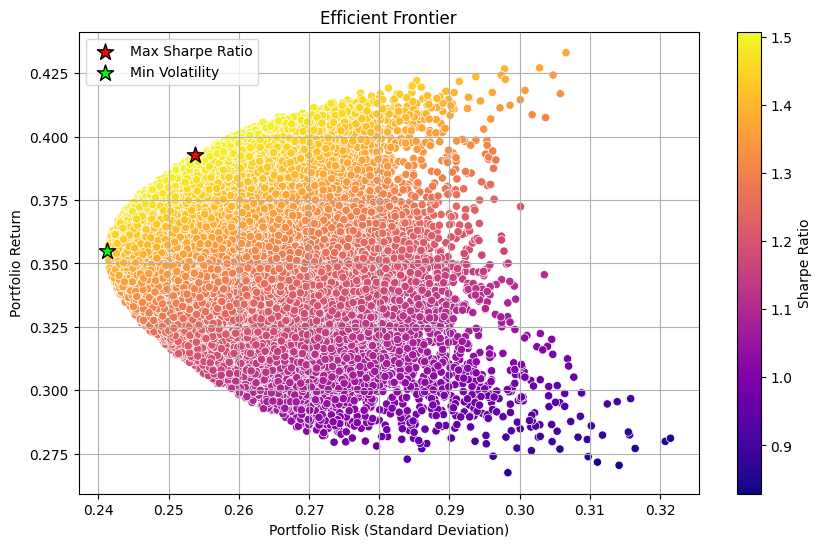
\includegraphics[width=0.8\linewidth,keepaspectratio]{Plots/EfficientFrontier.png}
	\caption{Efficient frontier with highlighted optimal portfolios}
	\label{fig:figure5}
  \end{figure}

Each point on the scatter plot represents a potential portfolio composed of 
the assets considered. The position of a point is determined by its risk (standard deviation 
on the $x$-axis) and expected return (on the $y$-axis).\newline \par \noindent The colour 
of each point corresponds to its Sharpe ratio, which measures the risk-adjusted return of the 
portfolio. A higher Sharpe ratio suggests a more favorable risk-to-reward trade-off. In this visualisation, 
the color gradient is shown using the plasma colormap, with warmer colours indicating higher 
Sharpe ratios. \newline \par \noindent A red star marks the portfolio with the maximum Sharpe 
ratio. It's the most desirable portfolio because it offers the highest return for a given level of 
risk. This point is often referred to as the \textit{tangency portfolio} since it's where the Capital 
Market Line or $CML$ (a line drawn from the risk-free rate tangent to the efficient frontier) touches the 
frontier.\newline \par \noindent Conversely, a lime star represents the portfolio with the minimum 
volatility (or risk). It's the safest portfolio because it has the lowest standard deviation, 
and thus, the lowest risk. \newline \par \noindent Lastly, the curve formed by the 
upper boundary of the scatter plot is what represents the efficient frontier. This boundary denotes the 
set of optimal portfolios that offer the highest expected return for a defined level of risk. 
Portfolios below this boundary are sub-optimal because they either provide less return for the same 
level of risk or have more risk for the same expected return.

\subsection{Optimised Portfolio Analysis}

\begin{tcolorbox}[colback=red!5, colframe=red!75!black, title=\textbf{Max Sharpe Ratio vs Min Risk}]

	The table below gives asset allocations for portfolios corresponding to the max Sharpe ratio and min risk. 
	The max Sharpe ratio portfolio aims to give the highest risk-adjusted return, and the min risk portfolio, 
	as the name suggests, aims to mitigate risk.

\begin{center}
		
		\begin{tabular}{|c|c|c|}
		\hline
		\textbf{Stock Ticker} & \textbf{Weight (Max Sharpe Ratio)} & \textbf{Weight (Min Risk)} \\
		\hline
		$AAPL$ & $0.214641$ & $0.003440$ \\
		\hline
		$GOOGL$ & $0.025050$ & $0.339532$ \\
		\hline
		$MSFT$ & $0.363010$ & $0.350740$ \\
		\hline
		$AMZN$ & $0.000673$ & $0.007854$ \\
		\hline
		$META$ & $0.396626$ & $0.298435$ \\
		\hline
		\end{tabular}

\end{center}

	As for the max Sharpe ratio portfolio, $META$ has the highest allocation of $39.66\%$, followed by $MSFT$ ($36.3\%$) 
	and then $AAPL$ ($21.46\%$). $GOOGL$ and $AMZN$ on the other hand, have much lower allocations of $2.51\%$ and 
	$0.07\%$ respectively. \newline \par \noindent For the min risk portfolio, $MSFT$ has the highest allocation 
	at $35.07\%$, closely followed by $GOOGL$ ($33.95\%$) and $META$ ($29.84\%$). $AAPL$ and $AMZN$ have minimal allocations, 
	at $0.34\%$ and $0.78\%$ respectively. \newline \par \noindent The asset allocation between the portfolios 
	is quite different, $META$ is heavily favoured in the max Sharpe ratio portfolio, but has a reduced weight in the min risk 
	portfolio. Conversely, $GOOGL$, which has a small presence in the max Sharpe ratio portfolio, has a significant weight in min 
	risk. $MSFT$ maintains a strong presence in both portfolios. $AMZN$ is minimally represented in both portfolios, 
	suggesting that, it might not be contributing substantially to either maximising the Sharpe ratio or minimising risk.
	
\begin{center}

		\begin{tabular}{|c|c|c|}
		\hline
		\textbf{Metric} & \textbf{Max Sharpe Ratio} & \textbf{Min Risk} \\
		\hline
		Portfolio Return & $0.396189$ & $0.353511$ \\
		\hline
		Portfolio Risk & $0.256094$ & $0.241258$ \\
		\hline
		Sharpe Ratio & $1.546296$ & $1.464490$ \\
		\hline
		\end{tabular}

	\end{center}
		
	The max Sharpe ratio portfolio has a ratio of $1.5463$, the portfolio return is $39.62\%$, 
	while the standard deviation is $25.61\%$. Comparing this with the min risk portfolio which has a 
	risk of $24.13\%$, a Sharpe ratio of $1.4645$ - just $0.0818$ difference, and a return of $35.35\%$. 
	It is clear that the max Sharpe ratio portfolio offers a higher expected return. This is consistent with the risk-return 
	trade-off; generally, portfolios with higher expected returns are also expected to exhibit higher 
	volatility (risk). \newline \par \noindent Similarly, the max Sharpe ratio portfolio has a slightly higher Sharpe ratio 
	than the min risk portfolio, suggesting that it provides a better risk-adjusted return. Lastly, for risk, as the name suggests, 
	the min risk portfolio has a lower volatility compared to the max Sharpe ratio portfolio, that said the difference in risk ($1.48\%$) 
	is not that substantial. \newline \par \noindent In summary, if maximising returns for a given level of 
	risk is the primary objective, then the max Sharpe ratio portfolio would be preferred. However, if minimising risk is more 
	crucial, even at the expense of higher returns, then min risk would be more suitable.

\end{tcolorbox}

Using the Sequential Least Squares Quadratic Programming ($SLSQP$) method, we are able to deduce the optimal allocation of capital 
across the five stocks to maximise the Sharpe ratio. More details in the \textbf{Jupyter Notebook}. \newline \par \noindent Apple 
accounts for approximately $22.07\%$ of the portfolio. Where as Google makes up $4.97\%$ of the portfolio. $SLSQP$ allocates 
roughly $34.78\%$ of the portfolio to Microsoft and $34.78\%$ to Meta (\textit{Facebook}). This means, based on the data and optimisation 
objective - Amazon's optimal weight is $0.00\%$ meaning it's not ideal to hold Amazon in the portfolio to achieve the maximum 
Sharpe ratio. \newline \par \noindent These weights suggest that the model finds the most value (in terms of risk-adjusted returns) 
in allocating capital to Meta and Microsoft. Apple also gets a significant allocation, while Google gets a smaller portion; and 
Amazon doesn't get any allocation under these parameters.

\section{Machine Learning in Portfolio Optimisation}

Portfolio optimisation has traditionally relied on mathematical models and techniques, 
such as the Capital Asset Pricing Model and Mean-Variance Optimisation, 
to determine the best allocation of assets in a portfolio. These traditional methods are 
based on certain assumptions about market behavior, which may not always hold true. 
This is where machine learning offers a fresh perspective. \newline \par \noindent Machine learning, 
with its ability to model and predict complex, non-linear relationships, provides tools to capture 
patterns in data that might be overlooked by traditional models. By analysing vast amounts of 
historical data, machine learning algorithms can identify intricate relationships between assets, 
potentially leading to better portfolio performance. \newline \par \noindent However, like all models, 
machine learning-based approaches have their limitations. They require large datasets to train on, 
can sometimes be opaque or hard to interpret (a challenge known as the \textit{black box} problem), and 
are sensitive to the quality of the input data.

\subsection{Machine Learning Algorithms Overview}

The three main machine learning models we'll be taking a look at are:

\begin{enumerate}

	\item Decision Trees: they map out decisions and their possible consequences. In portfolio 
		management, they can be used to decide on asset allocations based on certain criteria.
	
	\item Random Forests: an ensemble of Decision Trees, often trained with the bagging method. 
		They can reduce overfitting compared to a single Decision Tree and give better accuracy.
	
	\item Neural Networks: comprise layers of interconnected nodes or neurons. They are especially 
		good at capturing non-linear relationships in data, which can be beneficial for predicting stock 
		prices. (This model will be included in the \textbf{Jupyter Notebook}).

\end{enumerate}

To evaluate and compare the potential performance of different asset combinations, we'll simulate multiple 
portfolios with random asset allocations. This simulation will give us insights into the possible returns 
and volatilities we can expect from different portfolio structures. We'll simulate portfolios using 
historical data, and for each portfolio, we'll calculate its expected return and volatility based on 
the random asset weights. This will provide further insight into the risk-reward trade-off for our 
simulations. Then, in the following chapters, we will use the data gathered to train our $ML$ models.

\subsection{Decision Tree}

Decision Trees split the data into subsets based on certain decision rules - mapping out these decisions 
and their possible consequences. They are intuitive and easy to visualise but can sometimes overfit to the 
training data. A Decision Tree can be employed to predict the future return of a stock or a portfolio based 
on historical data. The tree makes decisions based on various factors, such as past returns, trading volumes, 
and other relevant financial indicators. \newline \par \noindent For our portfolio optimisation task, 
it's looking at relationships between asset weights, volatility, and returns to predict portfolio returns. 
The metrics we've computed provide insights into how well the Decision Tree has learned these relationships:

\begin{itemize}
	
	\item $MAE$ (Mean Absolute Error): this metric tells us, on average, how much our predictions deviate 
		from the actual returns. A lower $MAE$ is better.

	\item $RMSE$ (Root Mean Squared Error): this metric gives more weight to larger errors, making it more 
		sensitive to outliers than $MAE$. A lower $RMSE$ indicates a better fit to the data. Note $MSE$ is just
		the (positive) square root of the $RMSE$. We will explore $MSE$ later.
	
	\item $R$-squared: represents the proportion of the variance in the dependent variable that is 
		predictable from the independent variables. A value closer to $1$ indicates that the model 
		explains a higher proportion of the variance.

\end{itemize}

The process of hyperparameter tuning ensures that you're not just fitting your model to the training data but 
that it can also generalise well to unseen data. The hyperparameters are  set prior to training a machine 
learning model. They are not learned from the data but can significantly impact model performance. 
For example, certain hyperparameters can affect the speed and efficiency of training and can influence 
the complexity of the model leading to optimal model complexity. \newline \par \noindent In Decision Trees, 
the depth of the tree (\texttt{max\_depth}) can determine how well the model fits to the data. Too deep, and it may 
overfit; too shallow, and it may underfit. Some hyperparameters introduce regularisation (like the \texttt{min\_samples\_leaf} in 
Decision Trees), which can prevent overfitting by adding constraints to the model. \newline \par \noindent $k$-fold cross-validation 
involves partitioning the original training dataset into $k$ equal subsets or folds. Then, a model is 
trained using $k-1$ of the folds and validated on the remaining fold. This process is repeated $k$ times, 
with each fold serving as the validation set exactly once. The performance metric is then averaged over all $k$ 
trials to provide a more stable estimate of model performance. By integrating $k$-fold cross-validation in our 
Decision Tree training process, we ensure a more robust assessment of the model's capability. \newline \par \noindent In grid search, 
for each hyperparameter, we specify a range of values. The algorithm then systematically trains the model 
for every combination of hyperparameters. This ensures that we explore a wide range of configurations to 
find the best one. \newline \par \noindent To summarise, for each combination of hyperparameters, 
$k$-fold cross-validation trains the model on different subsets (or folds) of the data and validates it on 
the remaining data. This process is repeated $k$ times. This provides a more stable and robust estimate of 
the model's performance, ensuring that the chosen hyperparameters generalise well across different subsets 
of data.

\begin{tcolorbox}[colback=red!5, colframe=red!75!black, title=\textbf{Decision Tree Model Analysis}]

This is an explaination for the physical interpretations for each of the metrics calculated using the 
Decision Tree machine learning algorithm:

\begin{center}
	
	\begin{tabular}{|c|c|c|c|c|}
	\hline
	\textbf{Model} & \textbf{MAE} & \textbf{RMSE} & \textbf{$\textbf{R}$-squared} & \textbf{MSE} \\
	\hline
	Decision Tree & $0.001363$ & $0.001804$ & $0.967676$ & $0.000003$ \\
	\hline
	\end{tabular}

\end{center}

\begin{enumerate}

	\item $MAE$ (Mean Absolute Error): $\sim 1.36 \times 10^{-3}$ - this metric tells us that, on average, the 
		model's predictions are off by approximately $\sim 1.36 \times 10^{-3}$. Given that this is a small 
		value, it indicates the models predictions are quite close to the actual returns.

	\item $RMSE$ (Root Mean Squared Error): $\sim 1.80 \times 10^{-3}$ - $RMSE$ gives more weight to larger errors. 
		This means if you have more outliers or predictions that were way off, this value will increase. 
		The $RMSE$ being slightly higher than the $MAE$ suggests that there might be a few predictions where the 
		model didn't perform as well. Still, given the small value, the model is doing a good job overall.

	\item $R$-squared: $\sim 9.68 \times 10^{-1}$ - this is a proportion between  $0 \leq R^{2} \leq 1$, and it 
	tells you the percentage of the variance in the dependent variable (portfolio returns) that the 
	independent variables explain. An $R$-squared value of $\sim 9.68 \times 10^{-1}$ means that 
	$\sim 96.8\%$ of the variation in portfolio returns can be explained by the model. This is a strong 
	$R$-squared value, indicating a high level of predictive power.

	\item $MSE$ (Mean Squared Error): $\sim 3.00 \times 10^{-6}$ - this metric represents the average squared 
		difference between the observed actual out-turn values and the values predicted by the model. 
		The small $MSE$ value indicates that the model's predicitve capabilities are fairly accurate.

\end{enumerate}

\end{tcolorbox}

\subsection{Random Forest}

Random Forests are an ensemble learning method that builds upon the Decision Tree algorithm. 
Instead of relying on a single Decision Tree, Random Forests consist of multiple Decision Trees. 
A Random Forest uses a collection (or forest) of Decision Trees to make predictions, each tree 
is trained on a random subset of the data with replacement and makes its own predictions. This 
technique called bootstrapping, and means that some samples may be used multiple times in a 
single tree, while others may not be used at all. The Random Forest then aggregates these 
predictions to produce a final result which is typically an average of the predictions from all 
trees in the forest. This ensemble approach generally improves performance 
and reduces overfitting providing a more robust model compared to a single 
Decision Tree. \newline \par \noindent The benefits of using Random Forests in portfolio 
optimisation include the ability to capture complex, non-linear relationships between assets, 
as well as providing a measure of feature importance. This can be particularly useful 
in identifying which financial indicators or asset relationships are most influential in 
determining portfolio returns. \newline \par \noindent As with the Decision Tree model, 
we will evaluate the Random Forest's performance using the following metrics:

\begin{itemize}
	
	\item $MAE$: indicates the average error of the Random Forest model's predictions. Comparing 
		with Decision Tree's $MAE$ can give insight into the benefit of using ensemble.
 
	\item RMSE: helps understand the error distribution and the impact of outliers on the Random 
		Forest model's predictions. (We will cover $MSE$ later in the section).

	\item $R$-squared: a higher $R$-squared value would suggest that the ensemble of trees in the 
		Random Forest can explain more variance in the portfolio returns. 

\end{itemize}

\texttt{RandomizedSearchCV} is used for hyperparameter tuning, this is different from \texttt{GridSearchCV}
which was used in the Decision Tree model. The key difference being, traditional grid search methods evaluate 
every possible combination of hyperparameters, which can be computationally expensive. \texttt{RandomizedSearchCV}, 
on the other hand, samples a fixed number of hyperparameter combinations from the specified distributions. 
This approach is faster and can lead to better results, especially when the number of hyperparameters is large (as is the case).

\begin{tcolorbox}[colback=red!5, colframe=red!75!black, title=\textbf{Random Forest Model Analysis}]

This is an explaination for the physical interpretations for each of the metrics calculated using the 
Random Forest machine learning algorithm:
	
\begin{center}
		
	\begin{tabular}{|c|c|c|c|c|}
	\hline
	\textbf{Model} & \textbf{MAE} & \textbf{RMSE} & \textbf{$\textbf{R}$-squared} & \textbf{MSE} \\
	\hline
	Random Forest & $0.000536$ & $0.000763$ & $0.994220$ & $5.820780 \times 10^{-7}$ \\
	\hline
	\end{tabular}
	
\end{center}
	
\begin{enumerate}

	\item $MAE$ (Mean Absolute Error): $\sim 5.36 \times 10^{-4}$ - the $MAE$ for the Random Forest model is 
		approximately $\sim 5.36 \times 10^{-4}$. This metric conveys that, on average, the model's predictions 
		deviate by about $\sim 5.36 \times 10^{-4}$ from the actual values. Given the diminutive nature of this 
		value, it suggests that the Random Forest model's predictions are more precise compared to the 
		Decision Tree model, emphasising its heightened accuracy in forecasting returns.
	
	\item $RMSE$ (Root Mean Squared Error): $\sim 7.63 \times 10^{-4}$ - the $RMSE$ value is approximately 
		$\sim 7.63 \times 10^{-4}$. Like with the Decision Tree, the $RMSE$ metric prioritises larger errors more. 
		The fact that this value is slightly larger than the $MAE$, though still quite small, indicates there might 
		be occasional predictions where the model deviated a bit more. However, in general, the model's 
		performance is quite good.
	
	\item $R$-squared: $\sim 9.94 \times 10^{-1}$ - again, this metric represents the proportion of variance in 
		the dependent variable that can be attributed to the independent variables. An $R$-squared value of 
		$\sim 9.94 \times 10^{-1}$ denotes that around $\sim 99.4\%$ of the variation in portfolio returns is elucidated 
		by the model. This is an stronger $R$-squared value than the Decision Tree, showcasing the Random 
		Forest's superior predictive prowess.
	
	\item $MSE$ (Mean Squared Error): $\sim 5.82 \times 10^{-7}$ - again, the $MSE$ indicates the average squared discrepancy 
		between the observed actual outcomes and the values the model predicted. For the Random Forest, this value 
		is about $\sim 5.82 \times 10^{-7}$, which is significantly lower than that of the Decision Tree. This 
		underlines the Random Forest model's enhanced precision and suggests that the model has a strong capacity 
		to predict portfolio returns accurately.

\end{enumerate}

In summary, based on the provided metrics, the Random Forest model \textit{appears} to have a stronger predictive 
capability than the Decision Tree, with higher accuracy and precision in its predictions, we'll explore this further in the
next section.

\end{tcolorbox}

\section{Evaluating Machine Learning Model Performance}

The Random Forest model has a lower $MAE$ compared to Decision Tree, suggesting it makes, on average, smaller prediction 
errors compared to the Decision Tree model. Again, the Random Forest model has a lower $RMSE$, indicating it has fewer large 
prediction errors compared to the Decision Tree model. The $R^{2}$ value, often called the \textit{coefficient of determination}, is 
larger for the Random Forest model, meaning it can explain a larger portion of the variance in the returns compared to the Decision 
Tree model. Lastly, Random Forest outperforms the Decision Tree model with a significantly lower $MSE$ indicating better predictive 
accuracy. Based on these metrics and the rationale behind each of them, it is clear that the Random Forest model consistently outperforms 
the Decision Tree model. \newline \par \noindent However, it's essential to consider other factors like model interpretability, 
training time, and computational cost. While Random Forests might give better predictions, Decision Trees are simpler and more 
interpretable. \newline \par \noindent In summary, the Random Forest model, which utilises an ensemble of Decision Trees and 
aggregates their predictions, offers a more accurate and reliable prediction for portfolio returns in this 
context. \newline \par \noindent In the following sections, we will evaluate the performance of the $ML$ models by comparing 
the predicted against actual returns data, and investigate the impact of external factors on the feasibility of implementing $ML$-based 
strategies in a real-world scenario. 

\subsection{Impact of External Factors on ML Strategies}

\begin{tcolorbox}[title=\textbf{Feasibility of $ML$-based Models}]

	We will briefly outline and explore how external factors affect the performance and feasibility of 
	machine learning-based portfolio optimisation strategies.
	
	\begin{itemize}

		\item Transaction costs: high-frequency trading strategies based on machine learning can incur significant 
			transaction costs, which can erode profits. By simulating a trading strategy with and without transaction costs, 
			you can determine the impact on net returns.
		
		\item Market liquidity: machine learning models might identify arbitrage opportunities in illiquid stocks. 
			However, due to low liquidity, executing large trades can be challenging. Assessing the liquidity of assets 
			in the portfolio and comparing the model's performance on liquid verse illiquid assets can provide insights.

		\item Model complexity: while deep learning models can capture complex patterns, they require extensive 
			computational resources and can be prone to overfitting. Comparing the performance of a deep neural network 
			($DNN$) with a simpler model like linear regression or a Decision Tree can shed light on the trade-off between model 
			complexity and performance.

	\end{itemize}

	It's essential to consider transaction costs, market liquidity, and model complexity, as these can influence the 
	feasibility and effectiveness of machine learning models in a real-world scenario.

\end{tcolorbox}

\subsection{Training Data Analysis}

\begin{figure}[!htbp]
	\centering

	\begin{subfigure}[b]{0.8\linewidth}
		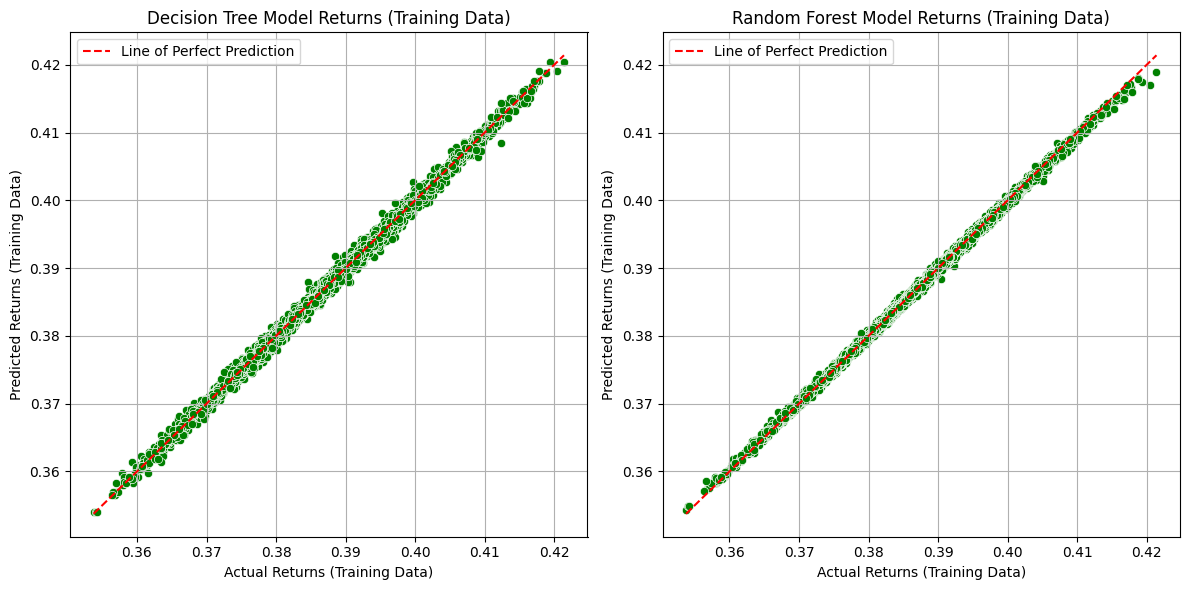
\includegraphics[width=\linewidth,keepaspectratio]{Plots/TrainingPvA.png}
		\caption{Predicted vs Actual Returns for the Training Dataset}
		\label{fig:figure6}
	\end{subfigure}
	
	\vspace{0.2cm} 
	
	\begin{subfigure}[b]{0.8\linewidth}
		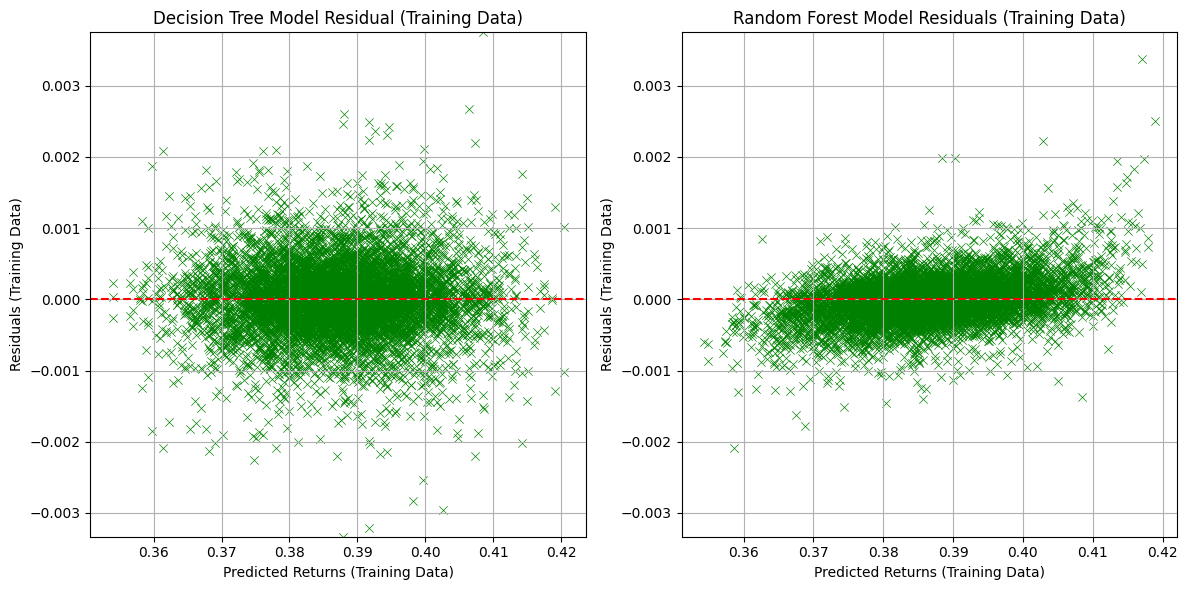
\includegraphics[width=\linewidth,keepaspectratio]{Plots/TrainingResidual.png}
		\caption{Residuals for DT and RF Training Dataset}
		\label{fig:figure7}
	\end{subfigure}
	
	\vspace{0.2cm} 
	
	\begin{subfigure}[b]{0.8\linewidth}
		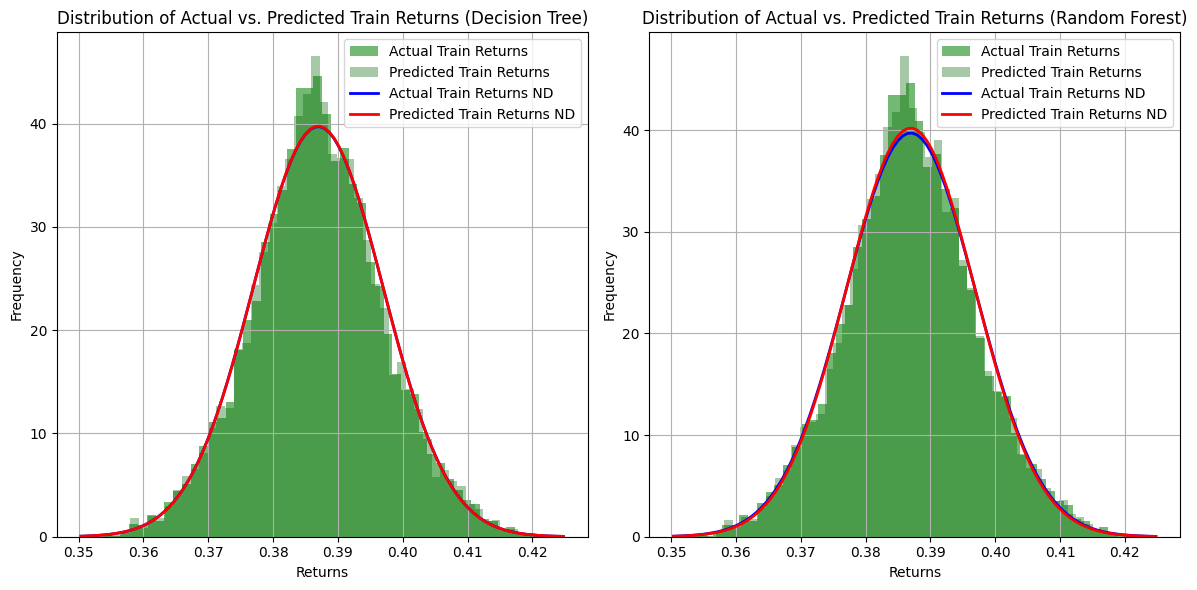
\includegraphics[width=\linewidth,keepaspectratio]{Plots/TrainingDistribution.png}
		\caption{Distribution for Actual vs Predicted Returns for the Training Dataset}
		\label{fig:figure8}
	\end{subfigure}
	
	\caption{Analysis of the Training Dataset for Decision Tree and Random Forest}
	\label{fig:combinedfigure1}

\end{figure}

\subsection{Validation Set Analysis}

\begin{figure}[!htbp]
	\centering

	\begin{subfigure}[!b]{0.8\linewidth}
		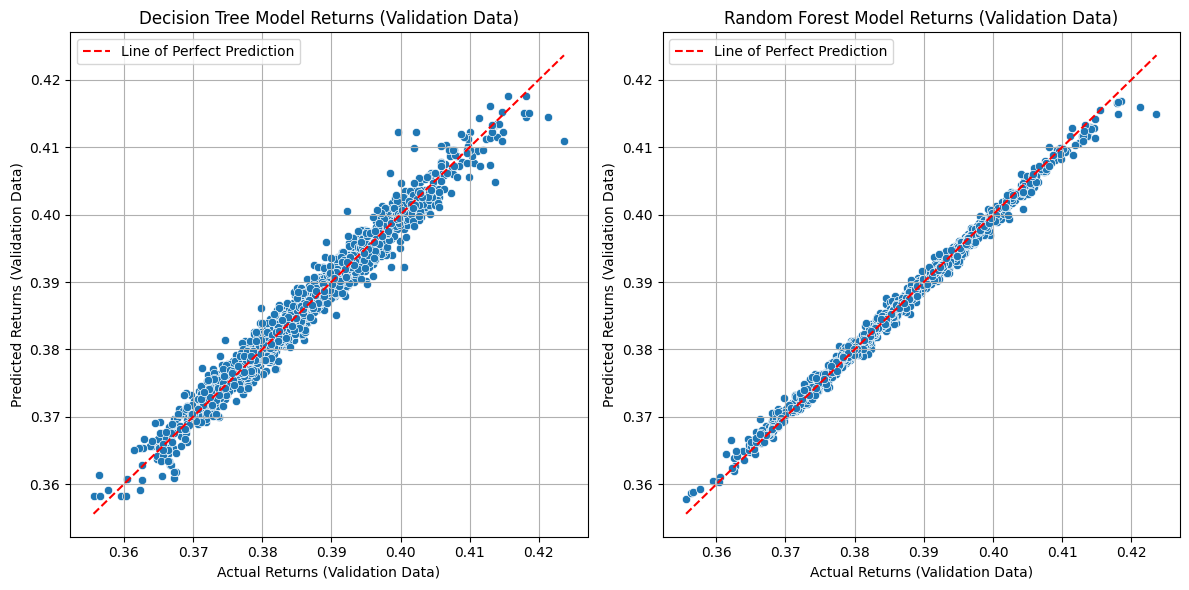
\includegraphics[width=\linewidth,keepaspectratio]{Plots/ValidationPvA.png}
		\caption{Predicted vs Actual Returns for the Validation Dataset}
		\label{fig:figure9}
	\end{subfigure}
	
	\vspace{0.2cm} 
	
	\begin{subfigure}[!b]{0.8\linewidth}
		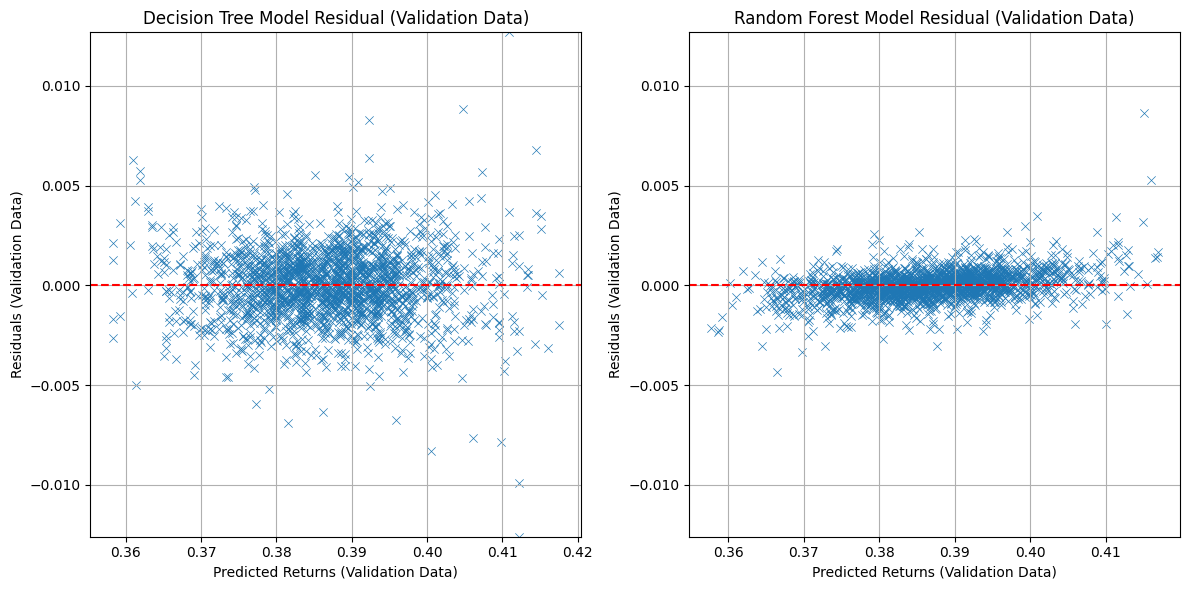
\includegraphics[width=\linewidth,keepaspectratio]{Plots/ValidationResidual.png}
		\caption{Residuals for DT and RF Validation Dataset}
		\label{fig:figure10}
	\end{subfigure}
	
	\vspace{0.2cm} 
	
	\begin{subfigure}[!b]{0.8\linewidth}
		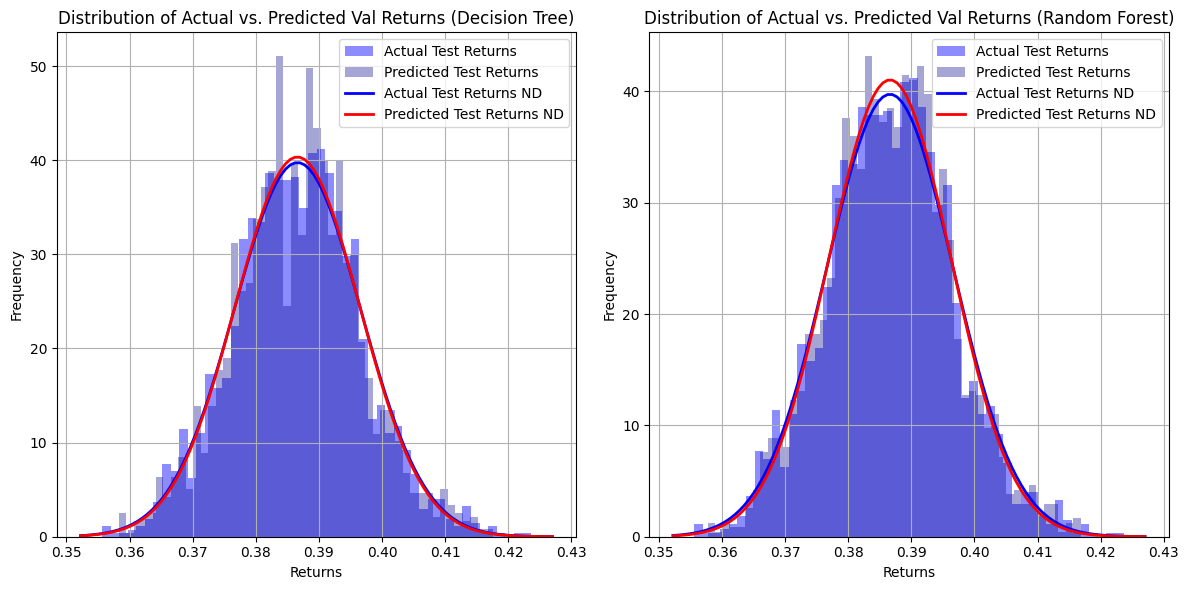
\includegraphics[width=\linewidth,keepaspectratio]{Plots/ValidationDistribution.png}
		\caption{Distribution for Actual vs Predicted Returns for the Validation Dataset}
		\label{fig:figure11}
	\end{subfigure}
	
	\caption{Analysis of the Validation Dataset for Decision Tree and Random Forest}
	\label{fig:combinedfigure2}

\end{figure}

\section{Future Research}

While this project explored traditional machine learning models like Decision Trees and Random Forests, the application 
of deep learning methods, such as recurrent neural networks ($RNN$s) or long short-term memory networks ($LSTM$s), could be 
valuable. These models have proven adept at capturing complex temporal patterns in data, which may be particularly relevant 
for financial time series. \newline \par \noindent Machine learning models such as Neural 
Networks are complex structures inspired by human brain function - they consist of layers of interconnected nodes 
or neurons. In fact, while we haven't talked much about Neural Networks, a $ML$ model has been implemented in the 
Jupyter Notebook \newline \par \noindent Incorporating alternative data, such as social media sentiment, macroeconomic indicators, 
or news analytics, could provide richer models. Understanding how these diverse data streams influence asset prices 
and portfolio performance can unveil novel investment strategies. \newline \par \noindent Lastly, rather than treating classical and machine 
learning models as separate entities, a hybrid approach that synergistically combines the strengths of methods like $CAPM$ 
or $MVO$ with machine learning could yield innovative strategies. An example might be, instead of simulating portfolios
with random asset weighting for Random Forests, we can use the optimised asset weights which were deduced using $MVO$.

\section{Conclusion}

This project embarked on an exploratory journey to understand the merging of portfolio optimisation and machine 
learning techniques, aiming to decipher whether machine learning offers a tangible advantage over traditional methods.
\newline \par \noindent Our analysis revealed that machine learning algorithms, particularly Random Forests, demonstrated 
a notable capability in capturing the non-linear relationships inherent in financial datasets. These models were able to 
unearth intricate patterns and dependencies which classical models might overlook. \newline \par \noindent Comparatively, 
while classical methods like Mean-Variance Optimisation and the Capital Asset Pricing Model 
offer a robust theoretical foundation, they come with underlying assumptions that may not always hold true in the 
chaotic world of financial markets. Whereas, machine learning models, 
with their data-driven approach, showed potential in navigating this chaos. \newline \par \noindent However, the integration 
of machine learning into portfolio management is not without its challenges. Considerations like transaction costs, market 
liquidity, and model complexity introduce layers of difficulty. Moreover, the black-box nature of many machine learning 
algorithms necessitates rigorous validation to ensure that they don't merely overfit historical data but genuinely offer 
predictive power. \newline \par \noindent This project underscores that machine learning, when wielded judiciously, can 
be a potent tool; and how it’s essential to approach this intersection of finance and technology with a balanced perspective, 
leveraging the strengths of both traditional financial models and advanced machine learning algorithms to achieve optimal 
portfolio performance.

\newpage
\bibliographystyle{plain}
\nocite{*}
\bibliography{references}

\end{document}